\documentclass{beamer}
\usepackage[russian]{babel}
\usetheme{metropolis}

\usepackage{adjustbox}
\usepackage{makecell}

\usepackage{amsthm}
\setbeamertemplate{theorems}[numbered]

\setbeamercolor{block title}{use=structure,fg=white,bg=gray!75!black}
\setbeamercolor{block body}{use=structure,fg=black,bg=gray!20!white}

\usepackage[T2A]{fontenc}
\usepackage[utf8]{inputenc}

\usepackage{hyphenat}
\usepackage{amsmath}
\usepackage{graphicx}

\AtBeginEnvironment{proof}{\renewcommand{\qedsymbol}{}}{}{}

\title{
Микроэкономика-I
}
\author{
Павел Андреянов, PhD
}

\begin{document}

\maketitle

\section{План}

\begin{frame}{План}

\begin{itemize}
  \item эффект дохода
  \item эффект замещения
  \item товар Гиффена
  \item матрица Слуцкого
\end{itemize}


\end{frame}


\section{Эффекты дохода и замещения}

\begin{frame}{Эффекты дохода и замещения}

Предположим, что цена на какой-то товар выросла $p \to p'$. 

Само по себе это еще не проблема, потому что потребители могли просто переключиться на ближайший субститут. Но могло случиться и так, что достаточно близкого субститута нет, и потребители все равно заплатили за дорогой товар 

Первая ситуация считается в каком-то смысле нормальной. Вторая - нет
\end{frame}

%%%%%%%%%%%%%%%

\begin{frame}{Эффекты дохода и замещения}

Попробуем формализовать эту идею. 

Изменение спроса можно разложить на два эффекта: эффект дохода и эффект замещения. Что это за эффекты?

\begin{itemize}
\item \alert{эффект замещения} (SE) – это <<катание>> бюджетной линии вдоль кривой безразличия
\item \alert{эффект дохода} (IE) – это <<параллельное смещение>> бюджетной линии
\end{itemize}

Почему всегда можно разложить? 

\end{frame}

\begin{frame}{Эффекты дохода и замещения}

\begin{figure}[hbt]
\centering
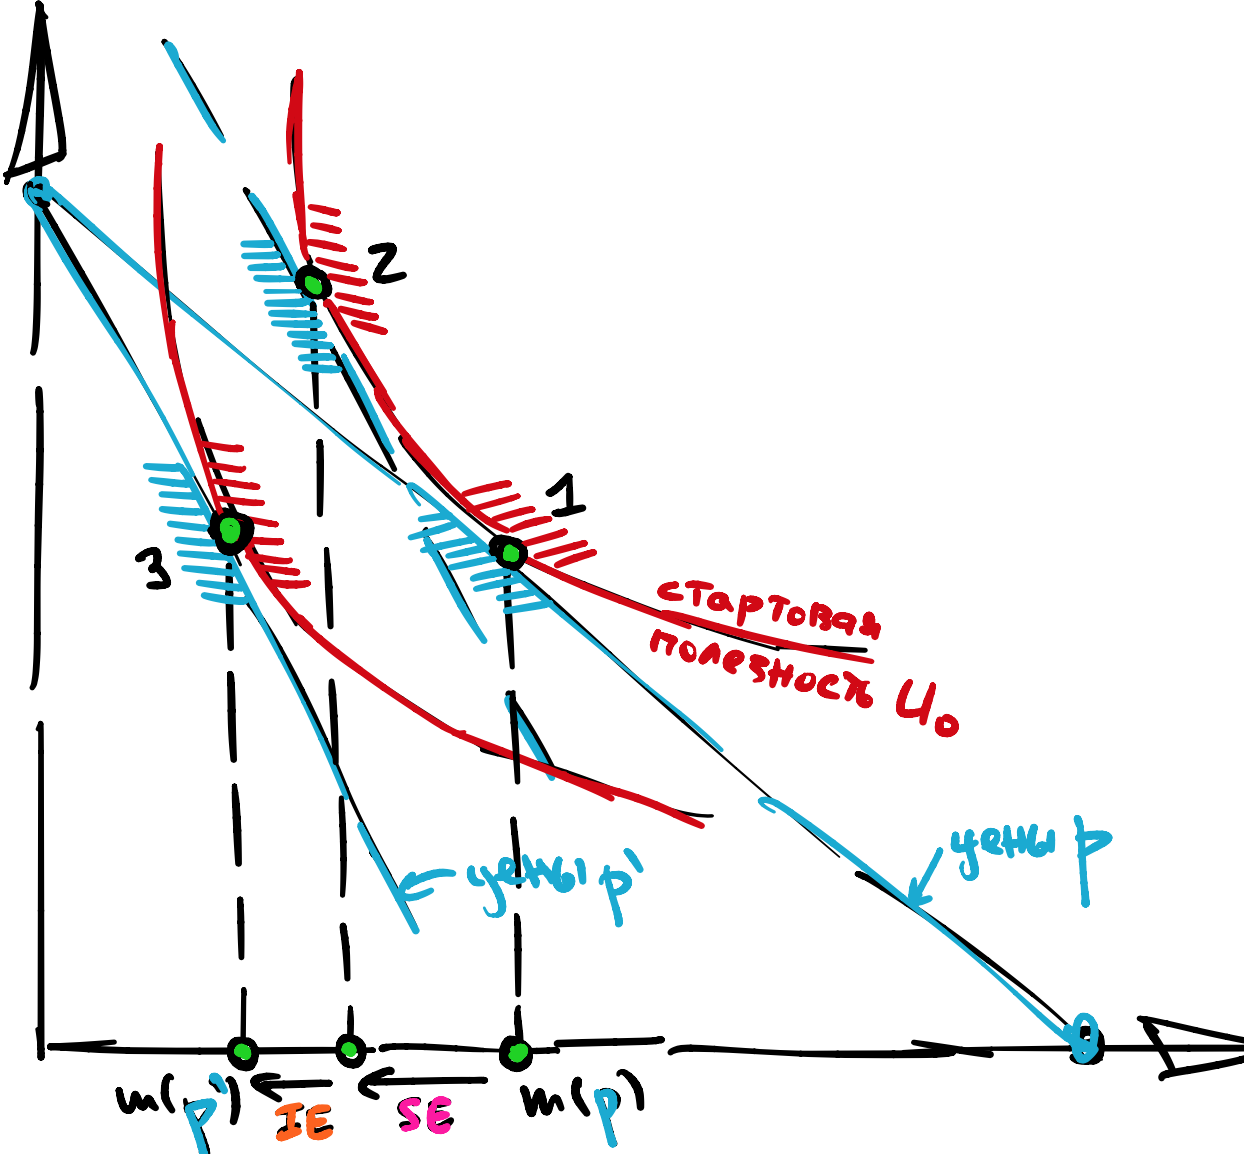
\includegraphics[width=.8 \textwidth]{SEIETE.png}
\end{figure}

\end{frame}

\begin{frame}{Общий эффект}

Есть также общий эффект (TE), он равен сумме эффекта замещения и эффекта дохода и представляет собой просто стандартное изменение маршаллианских спросов:
$$ \text{TE} = \text{SE} + \text{IE} = m(p') - m(p).$$

Поскольку маршаллианский спрос, как правило, наблюдаем, то можно считать, что общий эффект всегда известен. Неизвестно его разложение на эффект дохода и замещения.

\end{frame}

\section{Эффект замещения}

\begin{frame}{Эффект замещения}

Эффект замещения есть, по сути, приращение хиксианского спроса при полезности зафиксированной на изначальном уровне. 
$$ SE = h(p', \bar U_0) - h(p, \bar U_0) $$

Эффект замещения всегда отрицательный (неположительный, если быть точным), если он по своей цене, потому что мы доказали, что $\nabla^2 E \leqslant 0$.

\end{frame}

\begin{frame}{Эффект замещения}

\begin{figure}[hbt]
\centering
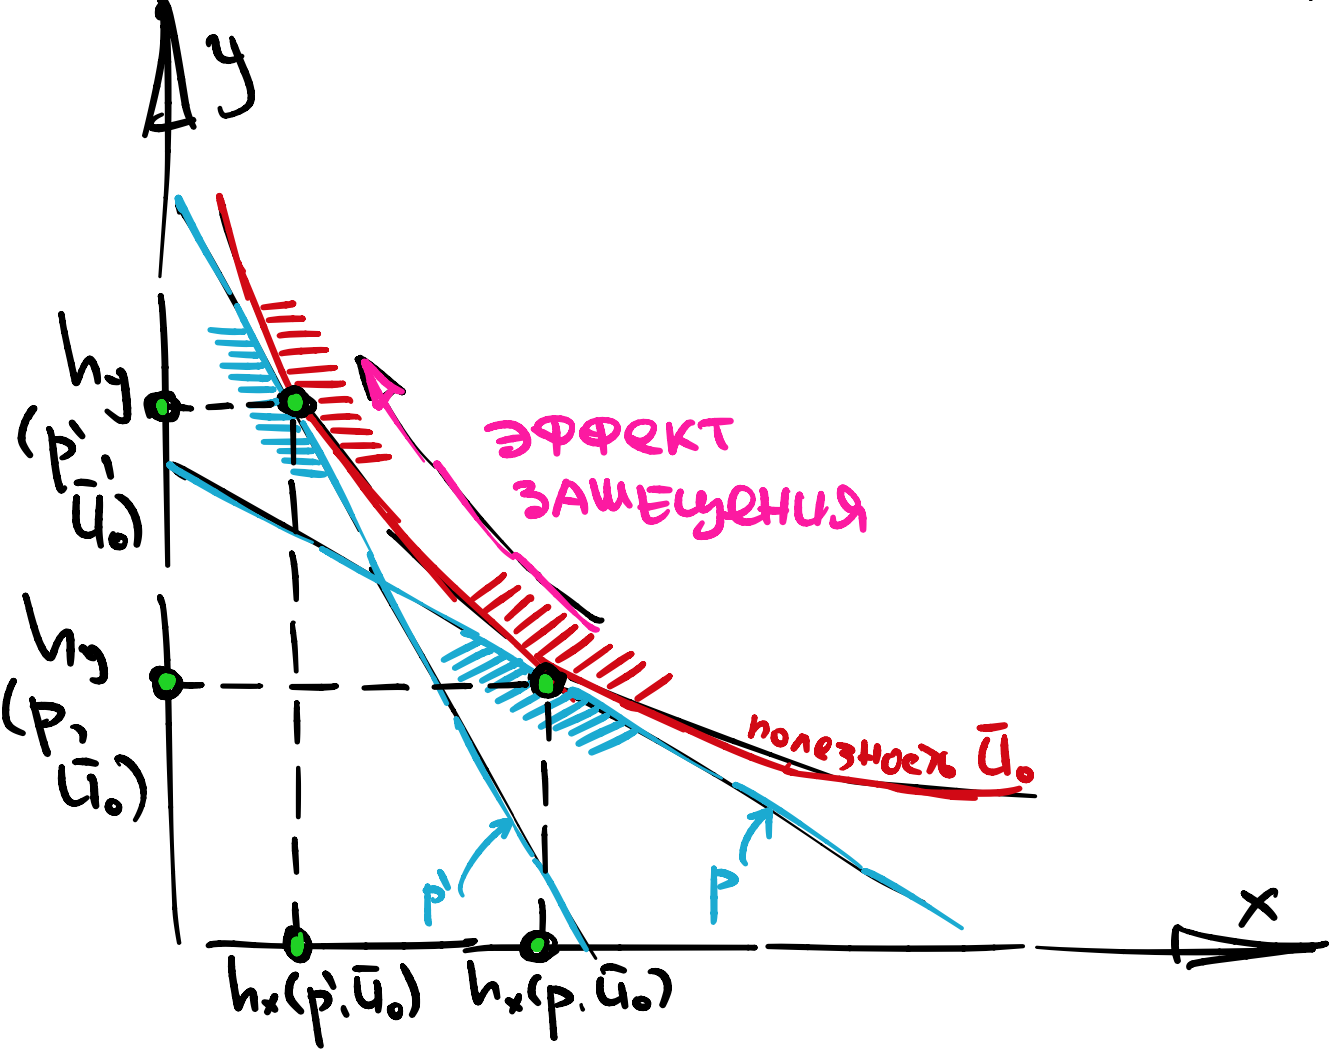
\includegraphics[width=.8 \textwidth]{SE.png}
\end{figure}

\end{frame}

\section{Эффект дохода}

\begin{frame}{Эффект дохода}

Эффект дохода есть разница между общим эффектом и эффектом замещения, именно так его надо считать. 

Эффект дохода IE меряет то, насколько повышение цены <<ограбило>> нашего агента. 

То есть, он служит той же цели что CV или EV. 

Только CV, EV - это числа а IE - это вектор.

\end{frame}

\begin{frame}{Эффект дохода}

\begin{figure}[hbt]
\centering
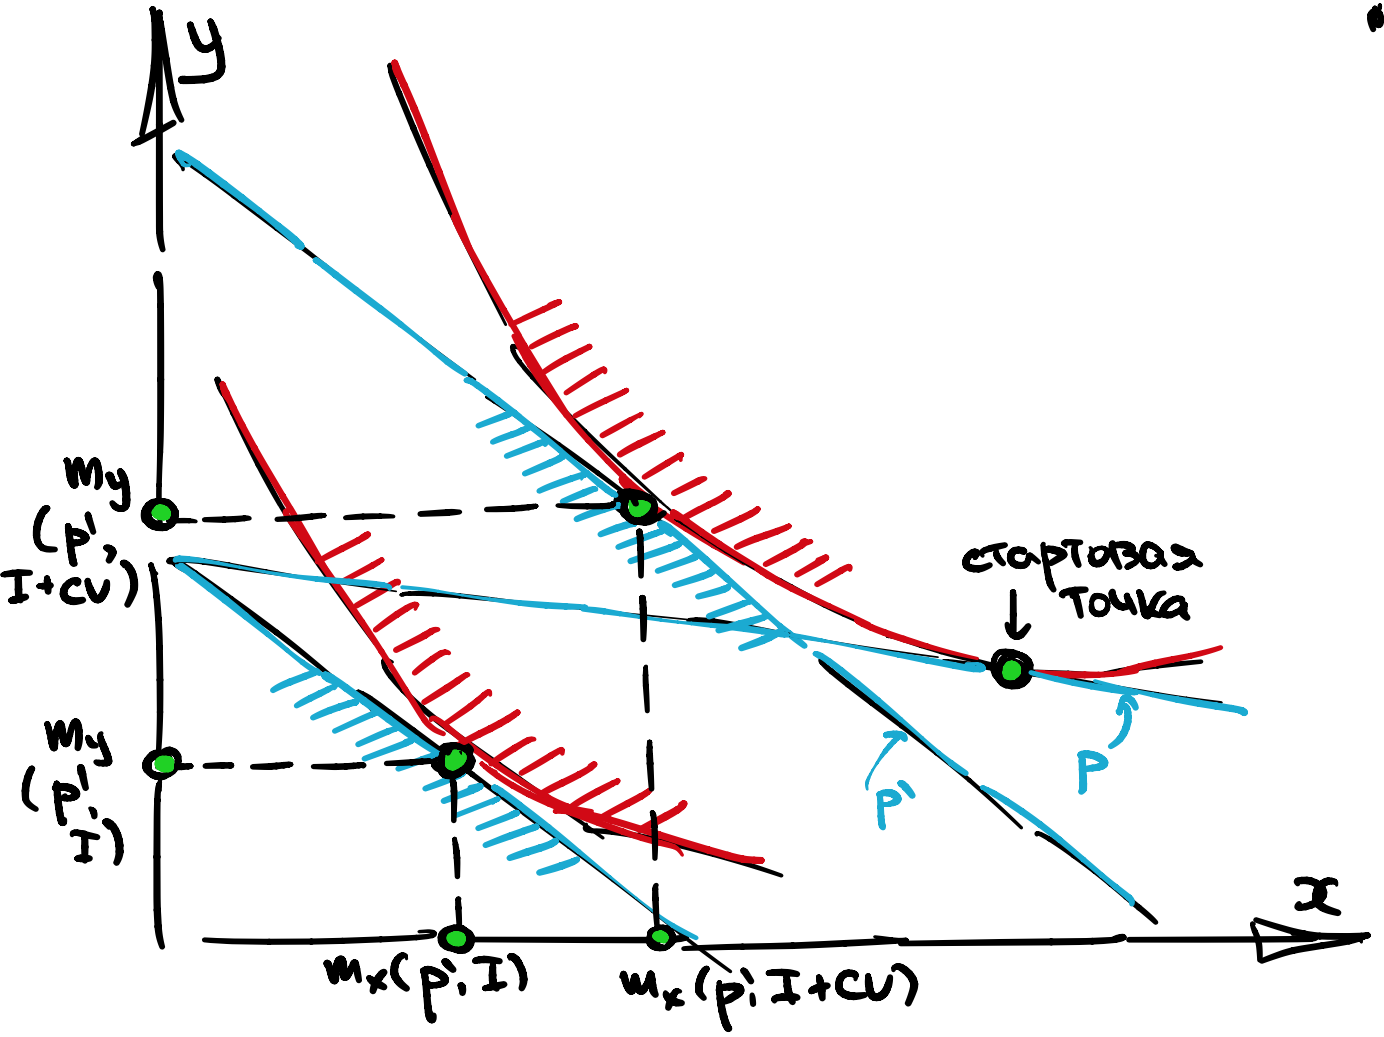
\includegraphics[width=.8 \textwidth]{IE.png}
\end{figure}

\end{frame}

\begin{frame}{Эффект дохода}
На самом деле, есть довольно простая связь между IE и CV.
$$ SE = h(p', U_0) - h(p, U_0), \quad TE = m(p',W) - m(p,W)$$
помним что IE это разница между TE и SE
\begin{eqnarray*}
IE & = & m(p', W) - h(p', U_0)\\
IE & = & m(p', W) - m(p', W + CV)\\
IE \cdot p' & = & m(p', W)\cdot p' - m(p', W + CV)\cdot p' \\
IE \cdot p' & = & W - (W + CV) = - CV
\end{eqnarray*}
То есть, |CV| это длина проекции IE на новый вектор цен.
\end{frame}


\begin{frame}{Эффект дохода}
Напомню что речь идет об изменении цен $p \to p'$.
\begin{itemize}
  \item Если у вас уже есть CV то эффект дохода это
  $$ IE = m(p', W) - m(p', W + CV)$$
  \item Если у вас уже есть IE то
  $$ CV = - IE \cdot p'$$
\end{itemize}
\end{frame}

\begin{frame}{Эффект дохода}

В отличие от эффекта замещения который всегда отрицательный по координате товара цена которого растет, эффект дохода может иметь более менее любой знак.

Попробуем нарисовать пример на доске, в котором эффект дохода будет положительным

\end{frame}

\begin{frame}{Эффект дохода}

Если эффект дохода положительный (не того знака что мы ожидаем), и довольно большой, то он может превзойти эффект замещения (у которого известный знак) так, что общий эффект будет положительный.

То есть, можно сделать так что цена на товар растет и его потребление растет. Это называется \alert{парадоксом Гиффена}.

Еще раз, эффект дохода и замещения направлены в противоположные стороны и эффект дохода побеждает.

\end{frame}

\begin{frame}
\begin{figure}[hbt]
\centering
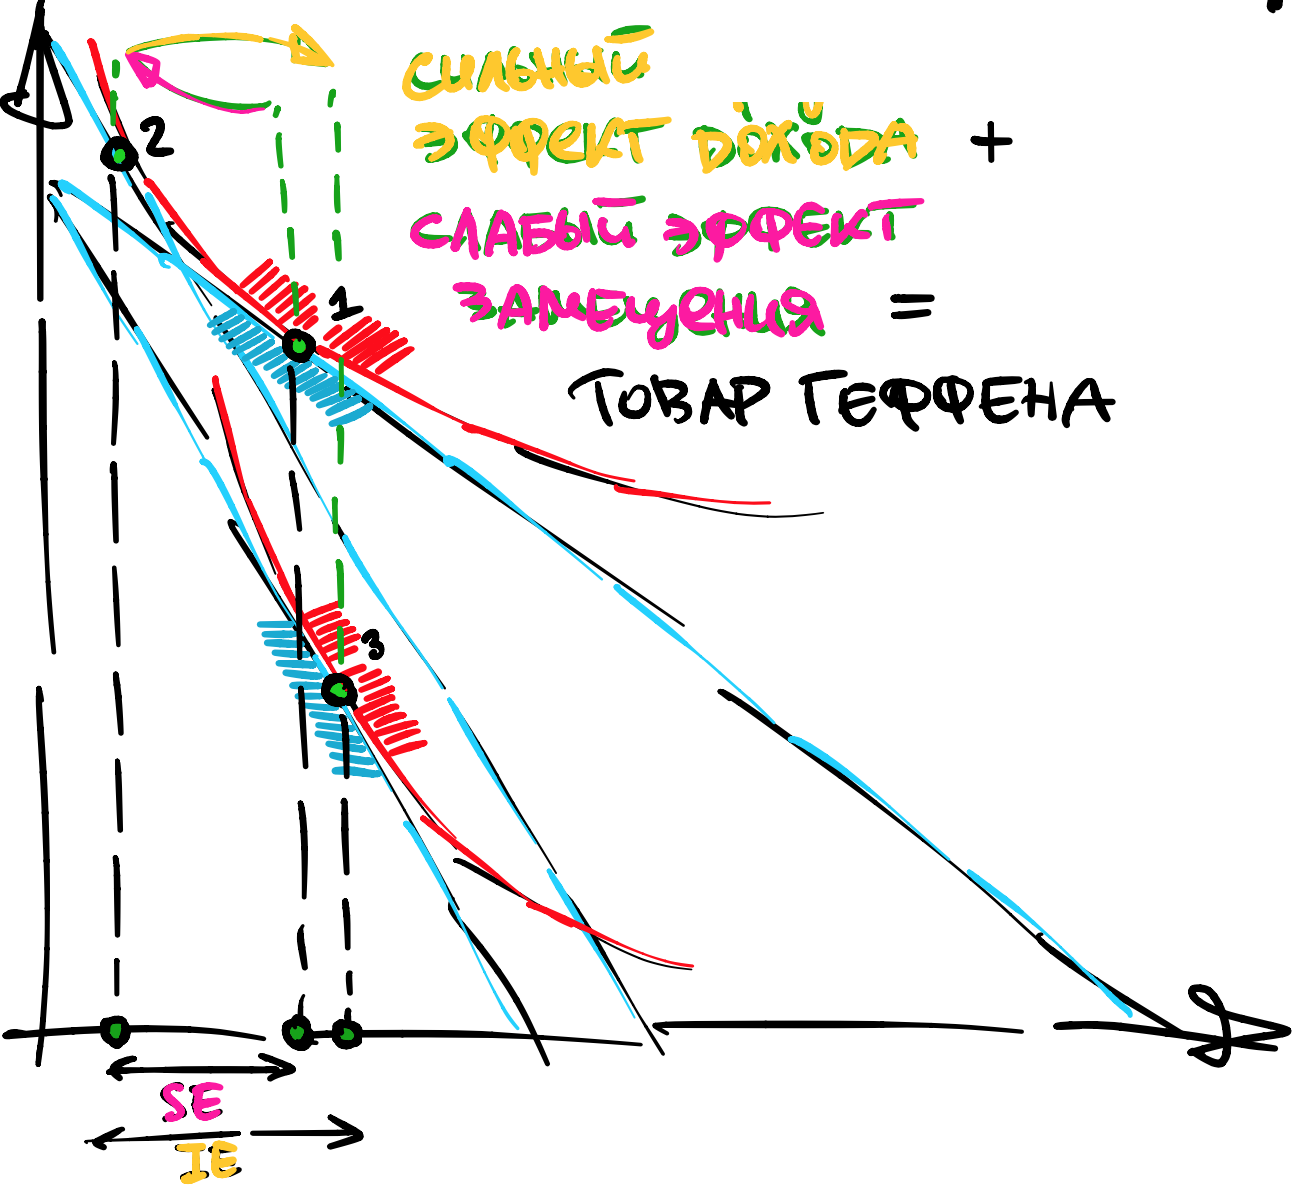
\includegraphics[width=.8 \textwidth]{IESE_CV.png}
\end{figure}

\end{frame}

\begin{frame}

Найдем IE у доски с кобб дугласом.

\end{frame}

\section{Матрица Слуцкого}

 \begin{frame}{Евгений Слуцкий}
 \begin{columns}
 \begin{column}{0.5\textwidth}
    \alert{Евгений Евгеньевич Слуцкий} советский математик и экономист начала 20 века. Из за него студенты экономики во всех университетах мира льют крокодиловы слезы, пытаясь понять его матрицы и уравнения.
 \end{column}
 \begin{column}{0.5\textwidth}  %%<--- here
     \begin{center}
      \includegraphics[width=1\textwidth]{eugen}
      \end{center}
 \end{column}
 \end{columns}
 \end{frame}
 
\begin{frame}{Евгений Слуцкий}
Матрица Слуцкого, она же матрица замещения, она же $S$ это просто гессиан функции расходов, который у нас фигурировал уже много где
$$ S = \nabla^2 E $$
Она описывает замещение. Что с ней можно делать?

Можно, например, разложить CV в ряд
$$ CV = E(p + \delta p) - E(p) \approx (\delta p) h + \frac{(\delta p) S (\delta p)}{2}$$
потому что $h = \nabla E$, а $S = \nabla^2 E$. (транспонирование расставьте самостоятельно так, чтобы получилось число)
\end{frame}

\begin{frame}{Матрица Слуцкого}
Матрица Слуцкого – это в некотором смысле четвертая модель поведения потребителя. То есть вместо калибровки полезности или предпочтений, мы можем калибровать матрицу замещения. 

Коэффициенты матрицы Слуцкого также можно переписать в терминах эластичности, дохода и долей, каждый из которых достаточно легко оценивается в данных. 
\end{frame}

\begin{frame}{Матрица Слуцкого}

Матрицу Слуцкого можно использовать для связи между хиксианскими и маршаллианскими эластичностями.

Сфокусируемся на уравнении, связывающем Хиксианский и Маршаллианский спросы:
$$\vec h (\vec p, \bar U) = \vec m(\vec p,  E(\vec p, \bar U)).$$

\end{frame}

\begin{frame}{Матрица Слуцкого}

Сфокусируемся на уравнении, связывающем Хиксианский и Маршаллианский спросы:
$$\vec h (\vec p, \bar U) = \vec m(\vec p,  E(\vec p, \bar U)).$$
Вас, скорее всего, не учили матричному дифференцированию, но в данном случае оно работает примерно как обычное:
$$ \nabla \vec h(\vec p,  \bar U) = \nabla \vec m(\vec p,  \bar U) + \frac{\partial m}{\partial I} \cdot \nabla E(\vec p, \bar U) = \nabla \vec m(\vec p,  \bar U) + \frac{\partial m}{\partial I} \cdot \vec h $$
Проблема в том, что и $\frac{\partial m}{\partial I}$ и $\vec h$ – это вектора длины $n$, и, поэтому, мы должны подумать, в каком порядке мы их хотим перемножить. 

\end{frame}

\begin{frame}{Матрица Слуцкого}

$$ \nabla \vec h(\vec p,  \bar U) = \nabla \vec m(\vec p,  \bar U) + \frac{\partial m}{\partial I} \cdot \vec h $$

Есть два варианта: либо мы умножаем строку $\frac{\partial m}{\partial I}$ на столбец $\vec h$, либо мы умножаем столбец $\frac{\partial m}{\partial I}$ на строку $\vec h$. 

Один из этих вариантов даст число, а другой – матрицу. Тот вариант, который сохранит размерность объекта, и будет правильным матричным дифференцированием. 

\end{frame}

\begin{frame}{Матрица Слуцкого}

В зависимости от того, что идет по строкам: координаты цен или координаты товаров – формула будет выглядеть по-разному. 

Например, если по горизонтали идут товары, то правильно:
$$ 
S = (\nabla h_x, \nabla h_y) = (\nabla m_x, \nabla m_y) + 
\begin{pmatrix} 
h_x \\
h_y
\end{pmatrix} 
\cdot (\frac{\partial m_x}{\partial I}, \frac{\partial m_y}{\partial I})
$$

Это называется \alert{уравнением Слуцкого}.

Чтобы не запутаться, достаточно запомнить, что вектор $h$ в правой части уравнения – это, на самом деле $\nabla_{\vec p} E$, то есть он относится к ценам, которые идут по вертикали.

\end{frame}

\begin{frame}{Матрица Слуцкого}

Далее, если $s_x$ и $s_y$ это доли товаров $x, y$ в бюджете, то верхний диагональный элемент уравнения Слуцкого можно записать как:
$$ \frac{\partial h_x}{\partial p} = \frac{m_x}{p} (\varepsilon_{x,p} + \varepsilon_{x,I} \cdot s_x)$$

А диагональный элемент уравнения Слуцкого можно записать как:
$$ \frac{\partial h_x}{\partial q} = \frac{m_x}{q} (\varepsilon_{x,q} + \varepsilon_{x,I} \cdot s_y)$$

К слову, эти уравнения связывают эластичности хиксианского и маршаллианских спросов.

\end{frame}

%\section{SE в первом приближении}
%
%\begin{frame}{SE в первом приближении}
%
%Матрица Слуцкого $S$ (она же $\nabla h=\nabla^2 E$) указывает нам на приращение Хиксианского спроса. 
%
%$$ SE = h(p') - h(p) = \int_p^{p'} \frac{\partial}{\partial p} h(x) dx \approx (p'-p) \nabla h = \delta p \cdot \nabla^2 E$$
%
%То есть если матрица оценена хорошо, то можно сказать, что приращение Хиксианского спроса – это приблизительно произведение матрицы Слуцкого на приращение цен. 
%
%А приращение Хиксианского спроса – это и есть $SE$.
%
%\end{frame}
%
%\section{Парадокс Гиффена}
%
%\begin{frame}
%
%Парадокс Гиффена заключается в том, что для некоторых товаров, которые пользовались популярностью у бедных: картофель и дешевый хлеб – наблюдалась прямая зависимость между ценой и спросом. Похожая зависимость иногда прослеживается для спроса на рис в современном Китае.
%
%Разрешение парадокса осуществляется за счет анализа Хиксианского спроса и матриц Слуцкого. 
%
%\end{frame}

\begin{frame}

Обратим внимание еще раз на эластичность Хиксианского спроса по собственной цене, которую я назову $\varepsilon^c_{x,p}$:
$$\varepsilon^c_{x,p} = \varepsilon_{x,p} + \varepsilon_{x,I} \cdot s_{x},$$

и перепишем ее так, чтобы маршаллианский спрос был слева:
$$\varepsilon_{x,p} = \varepsilon^c_{x,p} - \varepsilon_{x,I} \cdot s_{x}.$$

Легко видеть, что если $\varepsilon_{x,I} > 0$, то, поскольку $\varepsilon^c_{x,p}$ всегда неположительный, и $\varepsilon_{x,p}$ будет неположительный. И (локально) парадокс Гиффена не получится. 
\end{frame}

%\begin{frame}
%
%Соответственно, можно сделать следующий вывод:
%
%\textbf{Нормальный товар не объяснит парадокс Гиффена.}
%
%\end{frame}

\begin{frame}
Предположим, что товар $x$ инфериорный, то есть это товар низкого качества, тогда $\varepsilon_{x,I} < 0$. Предположим также, что доля товара $x$ в бюджете потребителя достаточно высока, то есть $s_{x}$ большой. Наконец, предположим, что для товара $x$ нет близкого (чистого) субститута, то есть $\varepsilon^c_{x,p}$ близок к нулю.

Тогда может так случиться, что $\varepsilon_{x,p}$ станет положительным.

\end{frame}

\begin{frame}
Еще раз
$$\varepsilon_{x,p} = \varepsilon^c_{x,p} - \varepsilon_{x,I} \cdot s_{x}.$$

\begin{itemize}
\item $s_{x}$ это доля
\item $\varepsilon^c_{x,p}$ это как бы эффект замещения
\item $\varepsilon_{x,I} \cdot s_{x}$ это как бы эффект дохода
\end{itemize}

Для того, чтобы объяснить парадокс Гиффена, нужно иметь слабый эффект замещения и сильный (за счет большой доли) отрицательный эффект дохода.

Одна картинка, обсудим примеры из жизни, и все.

\end{frame}

\begin{frame}
\begin{figure}[hbt]
\centering
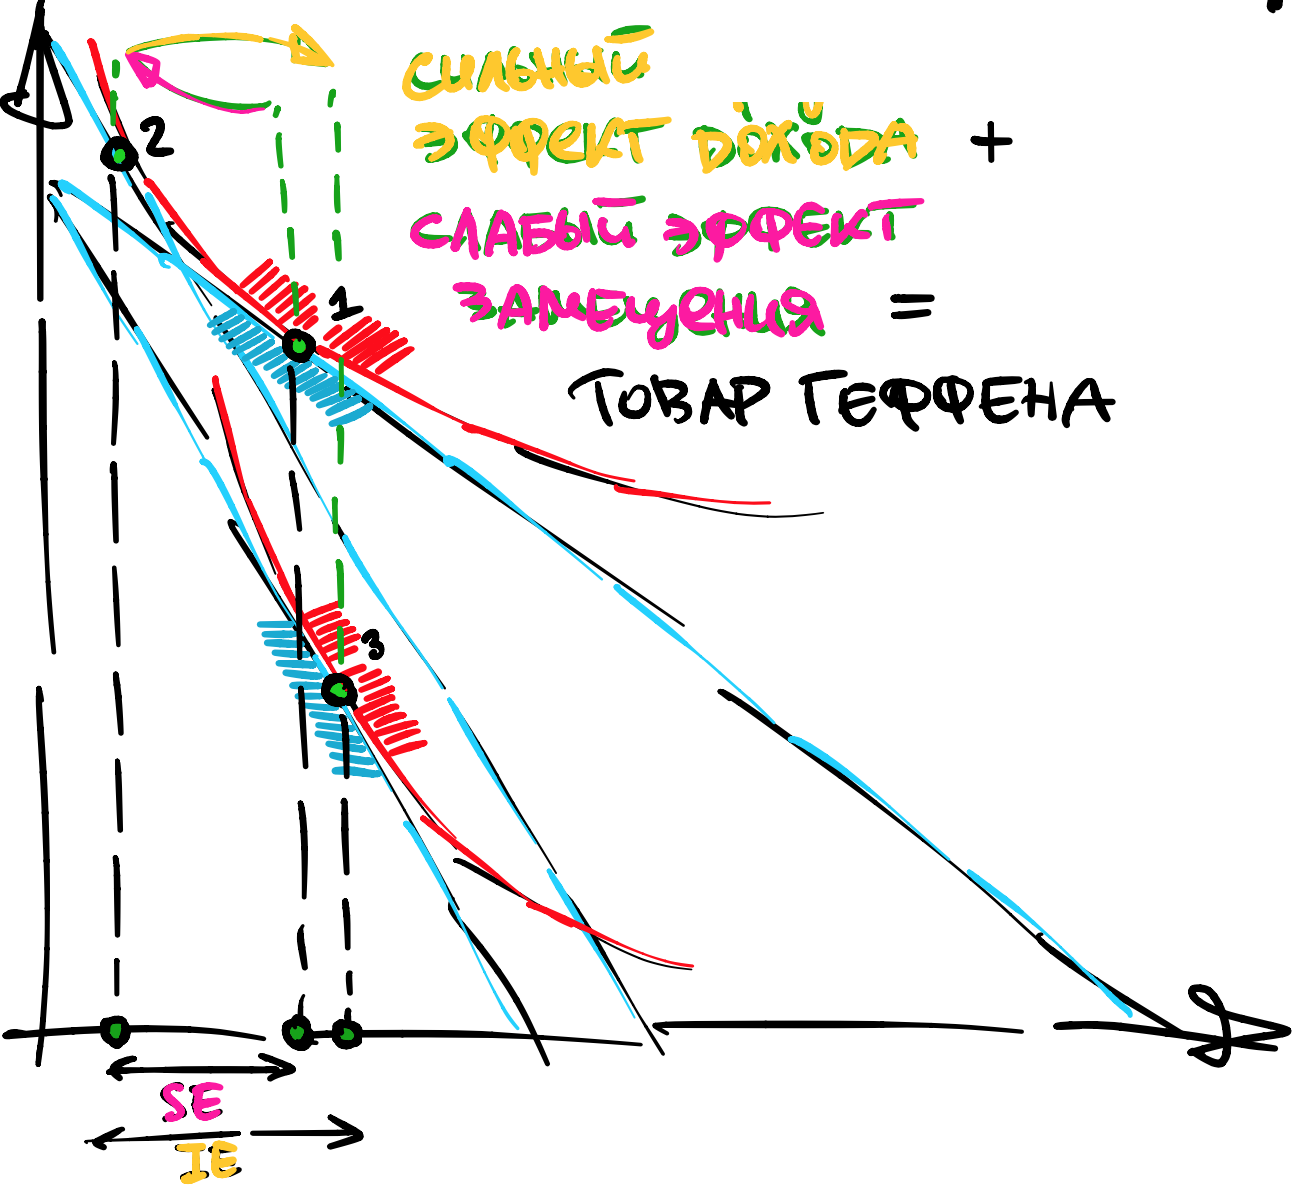
\includegraphics[width=.8 \textwidth]{IESE_CV.png}
\end{figure}

\end{frame}

\section{Это последняя лекция о теории потребителя}

\end{document}